\section{Diskussion}
\label{sec:Diskussion}
%Guck bitte nochmal über meine Kommentare... zumindest über die, wo ich nicht sicher war, ob ich verstanden habe, was du meinst. 

\subsection{Vorbereitung}
Bei der Justierung wird eine reale Eigenfrequenz von $\SI{33.1}{\kilo\hertz}$ gemessen. Mit einem Theoriewert von $f_+ = \sfrac{1}{2\pi\sqrt{L(C+C_{Sp})}} = \SI{30.5}{\kilo\hertz}$ ergibt dies eine
Abweichung von $\SI{2.6}{\kilo\hertz}$ bzw. $~8.5\%$.
Dies kann zum einen an abweichenden Angaben der Bauteile selbst liegen, %elliptische "Sätze" finde ich persönlicht nicht so wissenschaftlich ;)
zum anderen an der Genauigkeit der Messtechnik. Außerdem lässt sich der stufenlose Regler für die justierbare Kapazität $C$
nicht höher drehen, als es notwendig wäre; denn die am Oszilloskop abzulesende Lissajous-Figur erreicht nur annähernd einen Kreis. Somit sind die Kapazitäten der beiden 
Schwingkreise wesentlich unterschiedlich. Die bei der Durchführung kreisnaheste erreichte Lissajous-Figur ist in Abbildung \ref{fig:Lissajous} zu sehen.

\begin{figure}
    \centering
    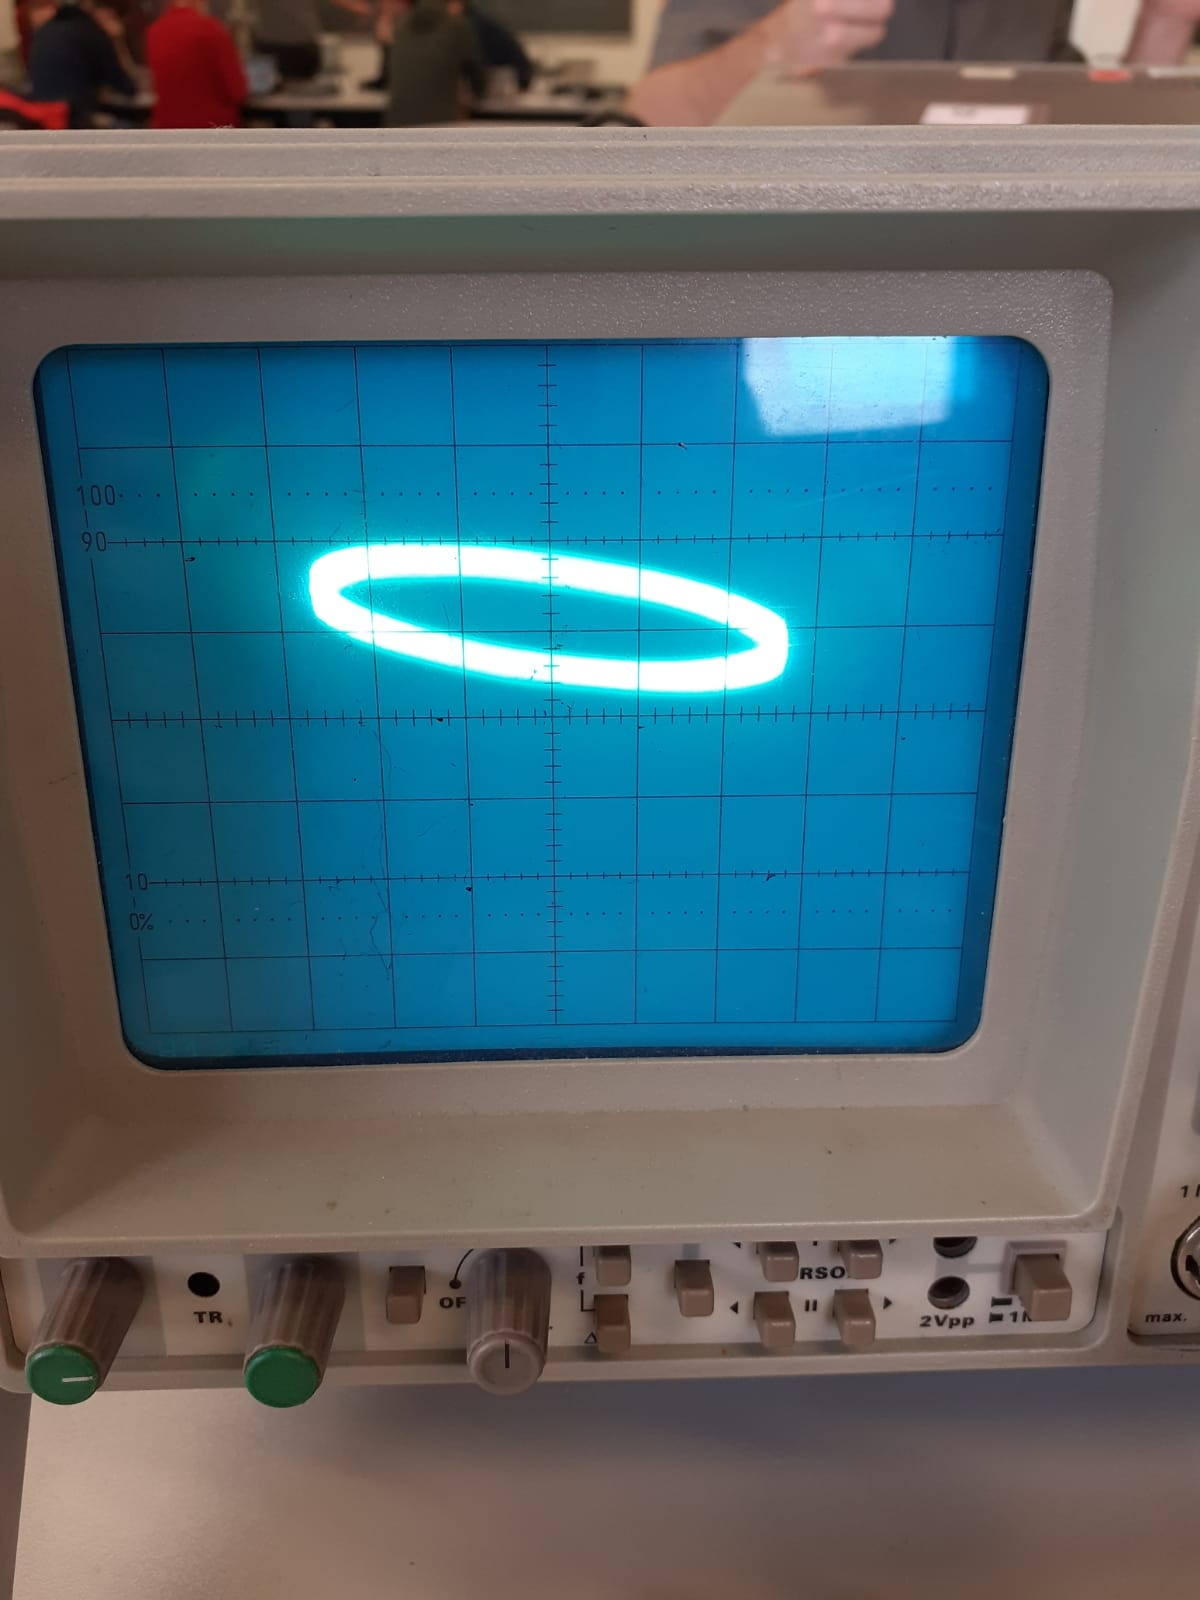
\includegraphics[width=0.75\textwidth]{plots/Lissajous_90Grad.jpeg}
    \caption{Lissajous-Figur der Justierung.}
    \label{fig:Lissajous}
\end{figure}

\subsection{Schwebung}
Eine Schwebung ist am Oszilloskop erst ab einer Kapazität von $C_K = \SI{4.7}{\kilo\hertz}$ ablesbar. Die Anzahl der Amplituden innerhalb einer Schwebungsperiode
steigt mit ansteigender Kapazität, was bedeutet, dass sich die überlagerten Frequenzen der gekoppelten Schwingkreise weiter annähern und die Differenz nach \eqref{eqn:fschwebung} geringer wird.
Wahrscheinlich liegt die Erklärung in der Koppelkapazität, welche einen Energieaustausch zwischen den beiden Systemen möglich macht. Hierdurch können die rückstellenden 
beziehungsweise %bzw. 
treibenden Kräfte
die Frequenzen der beiden Schwingkreise einander angleichen.
%Warum lässt sich nichts unter 4.7 nF ablesen? Frequenzen zu ähnlich + Messungenauigkeiten?

\begin{figure}
    \centering
    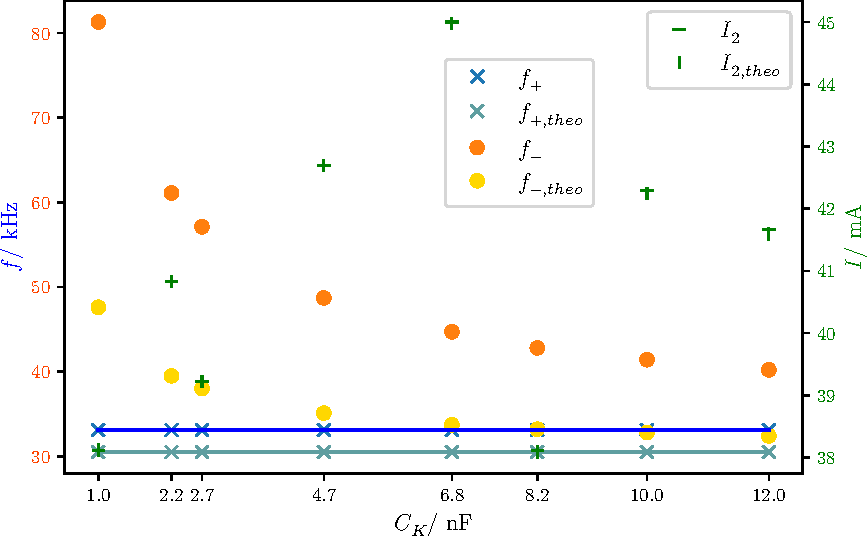
\includegraphics[width=0.85\textwidth]{plots/Messdaten_und_Theorie.pdf}
    \caption{Mess- und Theoriewerte im Vergleich.}
    \label{fig:mess_theo}
\end{figure}

\subsection{Resonanzfrequenzen}
Bei der Messung der Fundamentalschwingungen nimmt $f_+$ für alle Kapazitäten denselben Wert von $\SI{33.1}{\kilo\hertz}$ an. Dies entspricht genau der Erwartung,
da bei der ersten Fundamentalschwingung kein Strom durch $C_K$ fließt - und somit als normaler Leiter in dem Schaltkreis betrachtet wird.
Entgegen der Erwartung %jedoch -> ein antithetisches Wort reicht m.E. :) 
beträgt der Theoriewert $\SI{30.5}{\kilo\hertz}$. Wie bereits erwähnt werden hierbei entweder die Werte der Spule beziehungsweise des Kondensators höher sein.
Ungenauigkeiten in der Messtechnik können eine zusätzliche Fehlerquelle darstellen.

-- Für alle Vergleiche werden entweder Abbildung \ref{fig:mess_theo} oder Tabelle \ref{tab:theorie} betrachtet. --
%Für Spiegelstriche nicht Bindestrichte - sondern -- verwenden.. und ich glaube ein Leerzeichen zwischen Geschriebenem und Strich zur Formatierung braucht der auch noch

Die zweite %Konvention ist, Zahlen von eins bis zwölf auszuschreiben 
Fundamentalschwingung verhält sich vom Verlauf her wie vorhergesagt, dennoch weicht die Messung bei $C_K = \SI{1.0}{\nano\farad}$ um etwa $71\%$ ab.
Der %$\sfrac{1}{x}$-artige 
einer reziproken linearen Funktion ähnelnde Verlauf startet in der Theorie wesentlich tiefer und fällt deutlich langsamer. 
Die Werte, gegen die die Mess- und Theoriewerte konvergieren, liegen hingegen näher beieinander -- bei $C_K = \SI{12.0}{\nano\farad}$
und bei einer Abweichung von etwa $24\%$.
Solch eine Differenz lässt sich nur noch schwer durch abweichende Werte für Spule und Kondensator erklären. Der Kondensator $C_K$ wird mit einem Fehler von $\pm20\%$ angegeben.
Wird der Fehler maximal eingerechnet, ergibt sich für den ersten Wert von $C_K$ eine Kapazität von $\SI{1.2}{\nano\farad}$. 
%Folgenden Satz habe ich in deiner Fassung nicht ganz verstanden - also das was du sagen wolltest. Hab es jetzt umformuliert, hoffe sinngemäß deckt sich das einigermaßen
Der Abgleich aus der ersten Fundamentalschwingung von Mess- und Theoriewert legt die Annahme nahe, dass, wenn ${C_{ges} = C + C_{Sp} = \SI{0.8015}{\nano\farad} + \SI{0.037}{\nano\farad} = \SI{0.8385}{\nano\farad}}$ 
%ich glaube, es ist üblich, $$-Umgebungen in einer Zeile zu halten... wird gemacht, indem man am Anfang und am Ende jeweils { } setzt
ist, 
$L = \sfrac{1}{4\pi^2f_+^2C_{ges}} = \SI{4.57}{\milli\henry}$ sein müsste (im Vergleich zum angegebenen Wert von $L = \SI{32.351}{\milli\henry}$).
Selbst mit dem eingerechneten Fehler liegt die Resonanzfrequenz durch Einsetzen in \eqref{eqn:2nd_fund_Csp} sogar noch höher bei $f_- = \SI{120.7}{\kilo\hertz}$.
%Wenn du das hier liest: Guck bitte nochmal, ob du das wirklich für sinnvoll hältst, was du da in den letzten paar Zeilen geschrieben hast zu f_-... bin mir nicht sicher, was du meinst und dementsprechend auch nicht, ob das richtig ist

Eine Bewertung über die einzelnen Schaltkreiselemente ist also weder plausibel noch sinnvoll. Naheliegend ist ein systematischer Fehler, der erneut auf die Messtechnik zurückzuführen ist.
Außerdem können die Dämpfungseffekte durch den %ferrimagnetisch ist noch eine andere Form von Stoffmagnetismus ;)
ferromagnetischen Spulenkern ebenfalls die Messung beeinflussen. Die Ummagnetisierungsverluste sind jedoch zu gering, um derartige Abweichungen zu erklären.

\subsection{Ströme}
Die Erwartungswerte des Stromes $I_2$ liegen bemerkenswert nahe an den Messungen -- mit Abweichungen im Promille-Bereich. %hier eine Fehlerrechnung zu machen ist mir gerade zu blöd...
Das heißt, dass sowohl das Oszilloskop gut kalibriert ist, als auch dass die Angabe des Widerstandes mit $R = \SI{48}{\ohm}$ stimmt, sowie aber auch, dass der Generator die Spannung liefert, die er auch anzeigt.
Allerdings macht diese Genauigkeit keine Aussage über den Sinusgenerator der Spannungsquelle. Der mögliche systematische Fehler lässt sich also nur bedingt eingrenzen.

\subsection{Abschluss}
Die Schaltung 4, welche in diesem Versuch verwendet wird, ist durchaus fehlerbehaftet. Eine mögliche Verbesserung ist also das Austauschen oder Überprüfen dieses Schaltkreises.
Da das Oszilloskop die Spannung sehr genau angibt, kann hiermit gut gearbeitet werden. Es ist zudem sinnvoll vor dem Versuch %über das Oszilloskop zu prüfen,
mit dem Oszilloskop zu prüfen, %ich denke mal, du meintest diese Formulierung?
ob der Sinusgenerator die Frequenz erzeugt, die er angibt.
Wenn letzterer Abgleich erfolgreich ist, müssen systematische Fehler in der Schaltung liegen. 
%Konjunktiv 1 ("seien") wird hauptsächlich in der indirekten Rede benutzt (ansonsten laut Wikipedia noch im Jussiv (Aufforderung) und Optativ (Wunschformulierung)..)
Denkbar sind noch falsche Verkabelungen oder äußere Magnetfelder; diese sind aber auch als Erstes auszuschließen.
%Komma in Verbindung mit und/oder nur erlaubt, wenn das und/oder (Haupt-/Neben-)Sätze voneinander trennt
\pagebreak


%Zur Vorjustierung: Frage in der Anleitung beantworten: Wodurch können Abweichungen entstehen? (im vergleich von Messwert und berechneter Wert für Resonanzfrequenz) Wie genau wird der Messwert wohl sein? 
%Bei Bedarf: in \plots ist ein Bild, was für einen perfekten Kreis wir mit dem regelbaren Kondensator hinbekommen haben... eher eine Ellipse. Klar, man kann noch mit der Skalierung argumentieren... hier einfach als Fingerzeig, dass solch ein Bild existiert... sorry für die lange Zeile xD
